\documentclass[hyperref=colorlinks]{beamer}
\mode<presentation>
\usetheme{iclpt}
\setbeamertemplate{navigation symbols}{}
\setbeamertemplate{headline}{
%\setbeamercolor{institute in head/foot}{fg=beamer@iclightblue,bg=beamer@icmiddleblue}
%% \begin{beamercolorbox}[leftskip=.05\textwidth,rightskip=.05\textwidth,ht=.07\textheight,dp=0.1cm,wd=\textwidth]{institute in head/foot}
%% \end{beamercolorbox}
}
\setbeamertemplate{footline}{
%%\begin{beamercolorbox}[ht=.1\textheight,dp=0.4cm,wd=\textwidth,leftskip=3cm]{author in head/foot}%
  %% \begin{minipage}[c]{5cm}%
%%     \usebeamerfont{author in head/foot}
%%   \end{minipage}\hfill%
%%   \hfill
%%   \begin{minipage}{6cm}
%%     \hfill
%%   \end{minipage}
%%\end{beamercolorbox}%
}

\usepackage{color}
\usepackage{tabularx,colortbl}
\usepackage{graphicx}
\usepackage{pdfpages}
\usepackage{feynmp}
\usepackage[orientation=portrait,size=a1,scale=1.3,debug]{beamerposter}
\DeclareGraphicsRule{*}{mps}{*}{}

\title{}
%\subtitle{AN-12-403,PAS-HIG-13-013 \vspace{-0.7cm}}
\author{P. Dunne, Imperial College London}%{ D.Colling, \underline{P. Dunne}, A. Magnan, A. Nikitenko, J. Pela with \\ R. Aggleton, J. Brooke: Bristol \\ C.Asawangtrakuldee, Q.Li: Peking \\ P. Srimanobhas: Chulalongkorn \\ S. Kumar, K. Mazumdar: Mumbai}
\date{}

\begin{document}
\begin{fmffile}{feynmandiags}
  
  \section{Title}  
  \begin{frame}[t]
    \centering
    \vskip 1cm {\color{beamer@icdarkblue}\Huge Searches for Higgs decays to invisible final states at CMS}
    
    \begin{columns}
      \column{.2\textwidth}
      
\includegraphics[height=.04\textheight]{icl.pdf}       
      \column{.6\textwidth}
      \centering

      \huge {\color{beamer@icmiddlered} Patrick Dunne, pjd12@ic.ac.uk}
      \column{.2\textwidth}
      \hfill 
\includegraphics[height=.0425\textheight]{../Pics/CMS-Color.pdf}
    \end{columns}    
    
    
    \begin{block}{\centering \LARGE Why Higgs to invisible?}
      \begin{itemize}
        \large
        \centering
      \item The properties of the Higgs are not yet precisely measured.
      \item Many beyond the Standard Model theories predict invisible Higgs decays:
      \item[-] SUSY, extra dimensions, dark matter, etc.
        \vspace{.3cm}
        \vspace{.3cm}
      \end{itemize}
    \end{block}
    
    \begin{columns}
      \column{.59\textwidth}
      \begin{block}{\centering \LARGE How do you see something invisible?}
        \large
        \hspace{.3cm}
        \begin{itemize}
        \item Invisible particles still carry energy and momentum.
        \item Sometimes the Higgs is produced with other particles:
        \item[-] this is called associated production
        \item These other particles are used to infer the presence of a Higgs.
        \item The visible momentum is then summed and compared to the known total to infer the presence of invisible particles ($mE_{T}$).
        \end{itemize}
      \end{block}
      
      \column{.39\textwidth}
      
      \vspace{-.05cm}
      
      \begin{block}{\vspace{.2cm} \centering \LARGE Production channels \vspace{.15cm}}
        
        \begin{columns}
          \column{.49\textwidth}
          
          \centering
             \large VBF:
             
             \vspace{1.5cm}
             
             
             \centering
             
           \begin{fmfgraph*}(200,180)                                                                                              
             \fmfleft{i1,i2}                                                                                                                                  
             \fmfright{o1,o2,o3}                                                                                                                              
             \fmf{fermion}{i1,v1,o1}                                                                                                                          
             \fmf{fermion}{i2,v2,o3}                                                                                                                          
             \fmf{phantom,tension=4/5}{v1,v2}                                                                                                                 
             \fmffreeze                                                                                                                                       
             \fmf{photon,lab.side=right,label=$W,,Z$}{v1,v3}                                                                                                                 
             \fmf{photon,lab.side=left,label=$W,,Z$}{v2,v3}                                                                                                                
             \fmf{dashes}{v3,o2}                                                                                                                              
             \fmflabel{$q$}{i1}                                                                                                                               
             \fmflabel{$q$}{i2}                                                                                                                               
             \fmflabel{$q$}{o1}                                                                                                                               
             \fmflabel{$q$}{o3}                                                                                                                               
             \fmflabel{$H$}{o2}                                                                                                                               
           \end{fmfgraph*}
           
           \column{.49\textwidth}
           \centering
           \large ZH:
           
           \vspace{1.5cm}
           
           \centering
           \begin{fmfgraph*}(200,180)                                                                                                                                 
             \fmfleft{i1,i2}                                                                                                                                   
             \fmfright{o1,o2}                                                                                                                               
             \fmf{fermion}{i1,v1,i2}                                                                                                                           
             \fmf{photon,label=$Z$}{v1,v2}                                                                                                                  
             \fmf{photon}{v2,o1}                                                                                                                  
             \fmf{dashes}{v2,o2}                                                                                                                               
             \fmflabel{$q$}{i1}                                                                                                                                
             \fmflabel{$q$}{i2}                                                                                                                                
             \fmflabel{$Z$}{o1}                                                                                                                                
             \fmflabel{$H$}{o2}                                                                                                                                
           \end{fmfgraph*}
           \hspace{.25cm}
           
        \end{columns}
        
        \vspace{1.3cm}
      \end{block}
      
    \end{columns}

    \vspace{.1cm}

   
       \setbeamercolor{block body}{fg=beamer@iclightblue,bg=beamer@icmiddleblue}
      \begin{block}{}
        \centering
        \huge Searches in the VBF channel
      \end{block}
      \setbeamercolor{block body}{bg=beamer@iclightblue,fg=beamer@icdarkblue}
      \vspace{-1.2cm}
      \begin{columns}
        \column{.49\textwidth}%COLUMN 1
        \begin{minipage}[t][.365\textheight][t]{\linewidth}  
      
      \begin{block}{}
        \begin{itemize}
          \vspace{.3cm}
        \item VBF production has a distinctive topology and a high rate relative to ZH, making it the most promising channel:
        \item[-] The CMS expected limit on invisible branching fraction (BF(inv)) from VBF is 49\% compared to 83\% from ZH.
          \vspace{.3cm}
          \end{itemize}
      \end{block}

      \begin{block}{\centering \LARGE Strategy}
        \begin{itemize}
        \item Perform a simple counting experiment.
          \vspace{.3cm}
        \item Select distinctive VBF topology:
        \item[-] 2 jets with a large polar angle separation,
        \item[-] veto events with any other particles present.
          \vspace{.3cm}
        \item Require missing momentum to select the invisible final state.
          \vspace{.3cm}
          \item Use hard cuts to restrict backgrounds.
            \vspace{.3cm}
          \item Estimate remaining backgrounds.
            \vspace{.3cm}
        \end{itemize}
      \end{block}
      


      \begin{block}{\centering \LARGE Background estimation}
        \begin{itemize}
        \item We use a data driven method:
        \item[-] A control region enriched in background events is chosen,
        \item[-] The ratio between the signal and control regions from simulation is used to extrapolate to the signal region:

          \centering
          $N^{signal}_{Bkg} = (N^{control}_{obs}-N^{control}_{other bkgs}) \cdot \frac{N^{signal}_{Sim}}{N^{control}_{Sim}}.$
        \end{itemize}
      \vspace{.5cm}
      \end{block}
      \end{minipage}

      \column{.49\textwidth}%COLUMN 2
      \vspace{-.45cm}
      \begin{minipage}[t][.365\textheight][t]{\linewidth}

      \begin{block}{}
        \centering
        \vspace{0.0225\textwidth}
        
        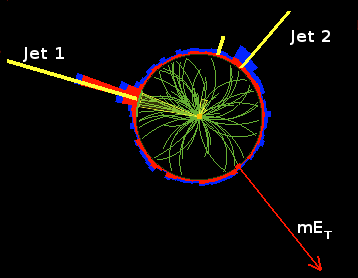
\includegraphics[width=.65\textwidth,trim=0 0 0 0]{Pictures/modifiedeventdisplay.png}
        
        \vspace{0.0225\textwidth}
      \end{block}



      \begin{block}{\centering \LARGE Main backgrounds}
        %\vspace{.4cm}
        \begin{columns}
          \column{.6\textwidth}
          \begin{itemize}
            \vspace{.3cm}
          \item $W$ + jets:
            \item[-] reduced by additional particle veto.
          \end{itemize}
          \column{.3\textwidth}
          %WJETS
          \hfill
          \begin{fmfgraph*}(150,120)
            \fmftop{i1,m1,m2,o1}
            \fmfbottom{i2,o2}
            \fmf{fermion,label=$e/\mu/\tau$,label.side=left}{v2,m1}
            \fmf{fermion,label=$\nu$,label.side=right}{v2,m2}
              \fmf{photon,tension=7/5,label=$W$}{v1,v2}
              \fmf{fermion}{v1,i2}
              \fmf{fermion}{v1,o2}
              \fmflabel{$jet$}{i2}
              \fmflabel{$jet$}{o2}
          \end{fmfgraph*}
          \column{.05\textwidth}
        \end{columns}
        
        %\vspace{.25cm}
        
        \begin{columns}
          \column{.6\textwidth}
          \begin{itemize}
          \item $Z\rightarrow\nu\nu$ + jets:
            \item[-] irreducible.
          \end{itemize}
          \column{.3\textwidth}
          %ZJETS
          \hfill
          \begin{fmfgraph*}(150,100)
            \fmftop{i1,m1,m2,o1}
            \fmfbottom{i2,o2}
            \fmf{fermion}{v1,i2}
            \fmf{fermion}{v1,o2}
            \fmf{photon,tension=7/5,label=$Z$}{v1,v2}
            \fmf{fermion,label=$\nu$,label.side=left}{v2,m1}
            \fmf{fermion,label=$\nu$,label.side=right}{v2,m2}
            \fmflabel{$jet$}{i2}
            \fmflabel{$jet$}{o2}
          \end{fmfgraph*}
          \column{.05\textwidth}
        \end{columns}

        %\vspace{.25cm}
        
        \begin{columns}
          \column{.6\textwidth}
          \begin{itemize}
          \item QCD multijets:
          \item[-] reduced by cuts.
          \end{itemize}
          \column{.3\textwidth}
          %QCD
          \hfill
          \begin{fmfgraph*}(150,120)
            \fmftop{i1,m1,m2,m3,m4,o1}
            \fmfbottom{i2,o2}
            \fmf{fermion,tension=4}{v1,i2}
            \fmf{fermion,tension=4}{v1,o2}
            \fmf{fermion,label=$jets$,label.side=left}{v1,m1}
            \fmf{fermion}{v1,m2}
            \fmf{fermion}{v1,m3}
            \fmf{fermion}{v1,m4}
            \fmflabel{$jet$}{i2}
            \fmflabel{$jet$}{o2}
          \end{fmfgraph*}
          \column{.05\textwidth}
        \end{columns}
        \vspace{.5cm}
      \end{block}

      \end{minipage}
      \vspace{.75cm}

      \end{columns}
%END OF FIRST SET OF VBF SEARCHES COLUMNS
      \vspace{-.1cm}
      \setbeamercolor{block body}{fg=beamer@iclightblue,bg=beamer@icmiddleblue}
      \begin{block}{}
        \centering
        \huge Results and future work
      \end{block}
      \setbeamercolor{block body}{bg=beamer@iclightblue,fg=beamer@icdarkblue}

      \vspace{-.3cm}
%START OF LAST SET OF COLUMNS
      \begin{columns}
        \column{.49\textwidth}%COLUMN 1
      \begin{minipage}[t][.365\textheight][t]{\linewidth}
      \begin{block}{}
        \vspace{.3cm}
        \begin{itemize}
          \vspace{.2cm}
        \item 2 other searches are performed at CMS in the ZH channel.
          \vspace{.2cm}
        \item Combining all 3 searches gives a limit of 58\% on invisible BF(inv) for a 125 GeV Higgs at 95\% C.L.:
        \item[-] strongest limit on BF(inv) of the Higgs to date,
        \item[-] compatible with the standard model at the 2$\sigma$ level.
          \vspace{.2cm} 
        \item We have additional 'parked' data with lower trigger thresholds that is yet to be analysed and more data will be taken starting in 2015:
        \item[-] this should give more events in our control regions and thus reduce the errors on our background estimation.
          \vspace{.2cm}
          %\item I would like to thank my supervisors David Colling and Gavin Davies and the members of my analysis group, particularly Anne-Marie Magnan and Andrew Gilbert, for the help they have given me, and the STFC for funding my work.
        \item More information can be found in arXiv:1404.1344.
          \vspace{.5cm}
        \end{itemize}
      \end{block}
      \end{minipage}

      \column{.49\textwidth}%COLUMN 2
      \begin{minipage}[t][.365\textheight][t]{\linewidth}
      \begin{block}{}
        \centering
        \includegraphics[width=.95\textwidth,height=.2\textheight,clip=true,trim=0 0 0 20]{Pictures/Combination-Limit.pdf}
      \end{block}
      \end{minipage}

      \end{columns}
      %\end{minipage}
    %\end{columns}
    \end{frame}
  
\end{fmffile}
\end{document}
